\section{Study Design}

In order to investigate whether amplitude or spatial based electrotactile feedback aids prosthetic control the most when removing the visual dependency, an experiment had been set up. A feedback coding scheme based on spatial activation and a feedback scheme based on amplitude modulation has been developed and will be presented later in \secref{ref til schmemes}. \\
XX subjects were recruited and randomly assigned to one of two groups. An overview of the total subject population and group demographics can be seen in \tabref{tab:demo}. Prior to enrollment, the subjects were assessed to meet the inclusion criteria stated in the experimental protocol, which can be found in \secref{Ex_protocol}. The subjects were handed the experimental protocol prior to the experiment session and gave an introduction to the background of the study and the different task the subjects would have to go through. Upon enrollment, the subjects were asked to sign an informed consent form (Fordi?). The experiment has been ethically approved by (Tilføj specifikationer).

\begin{table}[H]
	\caption{Overview of total subject population and group demographics.}\label{tab:demo}
	\begin{tabular}{llll} \hline
		& \textbf{Age, mean(std)} & \multicolumn{2}{c}{\textbf{Gender n(\%)}} \\ \cline{3-4}
		&                & Female          & Male           \\ \hline
		\begin{tabular}[c]{@{}l@{}}\textbf{Total}\\ (n = X)\end{tabular}   & \multicolumn{1}{c}{X(X)}    & X(X)       & X(X)      \\
		\begin{tabular}[c]{@{}l@{}}\textbf{Group 1}\\ (n = X)\end{tabular} & \multicolumn{1}{c}{X(X)}    & X(X)       & X(X)      \\
		\begin{tabular}[c]{@{}l@{}}\textbf{Group 2}\\ (n = X)\end{tabular}    & \multicolumn{1}{c}{X(X)}    & X(X)       & X(X)      \\ \hline
	\end{tabular}
\end{table}

The experiment was designed such that each subject was trained and tested in using both feedback schemes along with control during a one session experiment. A graphical illustration of the main stages that the subject went through can be seen in \figref{fig:std}. For all subjects data used to build the control system was acquired first. Secondly, the subjects were given time to familiarize with the control system and subsequently, the achieved control was assessed through a target reaching test. Finally, sensory thresholds used for feedback were determined for the subject. Subjects assigned to group 1 went through four steps of training and test using scheme 1 followed by the same four steps using scheme 2. The opposite was applicable for group two which started with scheme 2 followed by scheme 1. The next sections will further document the implementation and execution of the experiment.     

\begin{figure}[H]                 
	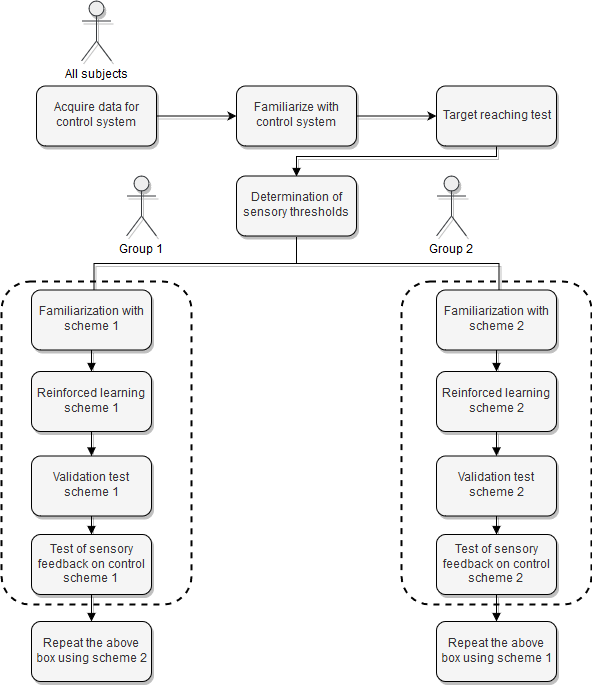
\includegraphics[width=.59\textwidth]{figures/std_design}
	\caption{Graphical illustration showing the stages of the experiment. Firstly, the stages common for all subjects followed by the group dependent stages.}
	\label{fig:std} 
\end{figure}